\documentclass[11pt]{article}

% Mandatory Packages
\usepackage{amsmath}
\usepackage{amssymb}
\usepackage{amsthm}
\usepackage{geometry}
\usepackage{tikz}
\usetikzlibrary{arrows.meta, positioning, shapes, fit, calc}
\usepackage{mathrsfs}
\usepackage{mathtools}
\usepackage{hyperref}
\usepackage{enumitem}
\usepackage{xcolor}

% Page Geometry
\geometry{letterpaper, margin=1in}

% Theorem Environments
\theoremstyle{definition}
\newtheorem{definition}{Definition}[section]
\newtheorem{axiom}{Axiom}[section]

\theoremstyle{plain}
\newtheorem{theorem}{Theorem}[section]
\newtheorem{lemma}[theorem]{Lemma}
\newtheorem{proposition}[theorem]{Proposition}
\newtheorem{corollary}[theorem]{Corollary}

\theoremstyle{remark}
\newtheorem{remark}{Remark}[section]

% Custom Commands for Probability and Set Theory
\newcommand{\R}{\mathbb{R}}
\newcommand{\N}{\mathbb{N}}
\newcommand{\Z}{\mathbb{Z}}
\newcommand{\Prob}{\mathbb{P}}
\newcommand{\E}{\mathbb{E}}
\newcommand{\F}{\mathcal{F}}
\newcommand{\sample}{\Omega}
\newcommand{\powerset}{\mathcal{P}}
\newcommand{\ind}{\mathbf{1}}

% Document Metadata
\title{\textbf{Homework 2: Tools for Counting Sample Points \\ \large Combinatorial Probability \& Measure Theory}}
\author{Tashfeen Omran}
\date{September 2026}

\begin{document}

\maketitle
\tableofcontents
\newpage

% ==============================================================================
% PART 1: Comprehensive Introduction, Context, and Prerequisites
% ==============================================================================
\section{Part 1: Comprehensive Introduction, Context, and Prerequisites}

\subsection{Core Concepts \& Axioms}
In the rigorous study of probability theory, we abandon informal notions of "chance" and replace them with precise measure-theoretic structures. A formal \textbf{Probability Space} is a triplet $(\sample, \F, \Prob)$, where:
\begin{enumerate}
    \item $\sample$ (Sample Space): A non-empty set of all possible fundamental outcomes $\omega$.
    \item $\F$ ($\sigma$-algebra): A collection of subsets of $\sample$ (events) that contains $\sample$, and is closed under complements and countable unions.
    \item $\Prob$ (Probability Measure): A function $\Prob : \F \to [0, 1]$ satisfying Kolmogorov's Axioms:
    \begin{itemize}
        \item $\Prob(\sample) = 1$ (Normalization).
        \item For any mutually exclusive sequence of events $\{E_i\}_{i=1}^{\infty}$ in $\F$, $\Prob\left(\bigcup_{i=1}^{\infty} E_i\right) = \sum_{i=1}^{\infty} \Prob(E_i)$ (Countable Additivity).
    \end{itemize}
\end{enumerate}

When dealing with finite, discrete, equiprobable sample spaces, the $\sigma$-algebra $\F$ is typically the power set $\powerset(\sample)$, and the probability measure is simply the \textbf{Counting Measure} normalized by the cardinality of $\sample$:
\[
\Prob(A) = \frac{|A|}{|\sample|} \quad \forall A \in \F
\]
The topic of \textit{Tools for Counting Sample Points} is fundamentally the mathematical discipline of \textbf{Combinatorics} acting as an evaluative mechanism for $|A|$ and $|\sample|$.

\subsection{Intuition and Set-Theoretic / Logical Foundations}
Combinatorial probability is the science of establishing bijections (one-to-one and onto mappings) between abstract event spaces and constructible sets (like sequences, partitions, or subsets). 
\begin{itemize}
    \item \textbf{Permutations ($P^n_r$):} Intuitively, these are injective functions mapping a set of $r$ distinguishable positions to a set of $n$ distinct objects. Order explicitly defines the mapping equivalence.
    \item \textbf{Combinations ($C^n_r$ or $\binom{n}{r}$):} These correspond to subsets of cardinality $r$ drawn from a set of cardinality $n$. Under the hood, this is a partitioning of the $n$ elements into two equivalence classes: "selected" and "unselected."
    \item \textbf{Multinomial Partitions:} This generalizes combinations. It evaluates the number of ways to define surjective mappings from $n$ distinct objects into $k$ distinct equivalence classes (groups) of predetermined sizes $n_1, n_2, \dots, n_k$.
\end{itemize}

\subsection{Historical Context and Motivation}
The foundational crisis of probability emerged in the 17th century when Blaise Pascal and Pierre de Fermat analyzed the "Problem of Points"—an interrupted gambling game. Prior to their correspondence, randomness was viewed philosophically or theologically. Pascal and Fermat developed algebraic structures (like Pascal's Triangle) to count discrete future trajectories of the game rigorously. Centuries later, Andrey Kolmogorov (1933) synthesized these combinatorial principles into the measure-theoretic axioms we use today, permanently binding discrete counting mechanisms with abstract real analysis and topology.

\subsection{Key Theorems, Lemmas, and Formulas}
\begin{theorem}[The $mn$ Rule / Fundamental Counting Principle]
If a set $\sample$ is formed by the Cartesian product $S_1 \times S_2 \times \dots \times S_k$, where $|S_i| = n_i$, then $|\sample| = \prod_{i=1}^k n_i$.
\end{theorem}

\begin{theorem}[Permutations]
The number of ordered injective sequences of length $r$ from $n$ distinct elements is:
\[
P^n_r = \frac{n!}{(n-r)!}
\]
\end{theorem}

\begin{theorem}[Combinations]
The number of subsets of cardinality $r$ from a set of cardinality $n$ is:
\[
\binom{n}{r} = C^n_r = \frac{n!}{r!(n-r)!}
\]
\end{theorem}

\begin{theorem}[Multinomial Partitions]
The number of ways to partition $n$ distinct objects into $k$ ordered groups of sizes $n_1, n_2, \dots, n_k$ (where $\sum n_i = n$) is:
\[
\binom{n}{n_1, n_2, \dots, n_k} = \frac{n!}{n_1! n_2! \dots n_k!}
\]
\end{theorem}

\subsection{Prerequisites}
To fully synthesize this material, one must possess a firm grasp of:
\begin{enumerate}
    \item \textbf{Naive Set Theory:} Union ($\cup$), Intersection ($\cap$), Complements ($A^c$), Cartesian Products ($\times$), and Cardinality ($| \cdot |$).
    \item \textbf{Algebraic Manipulations:} Expanding factorials ($n! = n \times (n-1)!$) and index-shifting in summations ($\sum$).
    \item \textbf{Proof Techniques:} Direct algebraic proof, combinatorial argument (proving identities by counting the same set in two different ways), and proof by induction.
\end{enumerate}

\newpage
% ==============================================================================
% PART 2: Detailed Homework Solutions (Rigorous Proofs & Computations)
% ==============================================================================
\section{Part 2: Detailed Homework Solutions}
\textit{Note: To maximize learning efficiency while reflecting every distinct archetype in the text, a strategic, fully representative subset covering mappings, combinations, multinomial partitions, and abstract identities has been selected.}

% --- Problem 2.39 ---
\subsection{Problem 2.39: Sum of Dice Mappings}
\textbf{Problem Statement:} An experiment consists of tossing a pair of dice. (a) Use combinatorial theorems to determine the number of sample points in $\sample$. (b) Find the probability that the sum of the numbers appearing on the dice is equal to 7.

\begin{proof}[Solution to 2.39]
\textbf{Part (a): Defining the Sample Space} \\
Let $D_1 = \{1, 2, 3, 4, 5, 6\}$ and $D_2 = \{1, 2, 3, 4, 5, 6\}$ represent the outcome spaces of the first and second die, respectively. The sample space is defined by the Cartesian product:
\[
\sample = D_1 \times D_2 = \{(i, j) \mid i \in D_1, j \in D_2\}
\]
By the \textit{Fundamental Counting Principle} ($mn$ rule) applied to Cartesian sets:
\[
|\sample| = |D_1| \times |D_2| = 6 \times 6 = 36 \text{ sample points.}
\]
\textbf{Part (b): Evaluating the Event Measure} \\
Let $A \subset \sample$ be the event where the sum of the dice equals 7. We define $A$ via set-builder notation:
\[
A = \{(i, j) \in \sample \mid i + j = 7\}
\]
Because $j = 7 - i$, and we require $1 \le j \le 6$, we substitute to find bounds for $i$:
\[
1 \le 7 - i \le 6 \implies -6 \le -i \le -1 \implies 1 \le i \le 6
\]
For each $i \in \{1, 2, 3, 4, 5, 6\}$, there exists exactly one $j$ satisfying the condition. The bijection yields the elements:
\[
A = \{(1,6), (2,5), (3,4), (4,3), (5,2), (6,1)\} \implies |A| = 6
\]
Assuming the dice are fair, the probability measure $\Prob$ is discrete uniform. Thus:
\[
\Prob(A) = \frac{|A|}{|\sample|} = \frac{6}{36} = \frac{1}{6}
\]
\end{proof}

% --- Problem 2.44 ---
\subsection{Problem 2.44: Abstract Multinomial Partitions (Taxis)}
\textbf{Problem Statement:} A fleet of nine taxis is dispatched to three airports: 3 to A, 5 to B, and 1 to C. Assume assignments are random. (a) If exactly one taxi needs repair, what is the probability it is dispatched to C? (b) If exactly three need repair, what is the probability every airport gets one?

\begin{proof}[Solution to 2.44]
\textbf{Sample Space Setup:} \\
We partition $n = 9$ distinct taxis into $k = 3$ sets (airports A, B, C) with specific cardinalities $n_1=3, n_2=5, n_3=1$. The total number of valid partitions is the multinomial coefficient:
\[
|\sample| = \binom{9}{3, 5, 1} = \frac{9!}{3! 5! 1!} = \frac{9 \times 8 \times 7 \times 6 \times 5!}{6 \times 5! \times 1} = 504
\]
Since assignments are random, $\Prob(\{\omega\}) = 1/504$ for all $\omega \in \sample$.

\textbf{Part (a): Single Defect Partition} \\
Let $E_1$ be the event the repaired taxi is sent to airport C. We decompose the fleet into two sets: \{Repaired Taxi ($R$)\} (size 1) and \{Functional Taxis ($F$)\} (size 8). 
To satisfy $E_1$, $R$ must be assigned to C. This leaves 0 spots in C, 3 in A, and 5 in B for the remaining 8 functional taxis. We partition $F$:
\[
|E_1| = \binom{1}{0,0,1} \times \binom{8}{3,5,0} = 1 \times \frac{8!}{3! 5! 0!} = \frac{8 \times 7 \times 6}{6} = 56
\]
\[
\Prob(E_1) = \frac{|E_1|}{|\sample|} = \frac{56}{504} = \frac{1}{9}
\]

\textbf{Part (b): Triple Defect Uniform Distribution} \\
Let $E_3$ be the event that exactly three taxis are broken, and each airport receives exactly one. We partition the fleet into $R$ (size 3) and $F$ (size 6). 
To satisfy $E_3$, the 3 elements of $R$ must be partitioned into subsets of sizes $1, 1, 1$ for A, B, C. The remaining 6 elements of $F$ must fill the remaining capacities: $3-1=2$ for A, $5-1=4$ for B, and $1-1=0$ for C. Using the fundamental counting principle on independent partitions:
\[
|E_3| = \binom{3}{1,1,1} \times \binom{6}{2,4,0} = \frac{3!}{1!1!1!} \times \frac{6!}{2!4!0!} = 6 \times 15 = 90
\]
\[
\Prob(E_3) = \frac{|E_3|}{|\sample|} = \frac{90}{504} = \frac{5}{28} \approx 0.1786
\]
\end{proof}

% --- Problem 2.45 ---
\subsection{Problem 2.45: Multinomial Algebraic Expansion}
\textbf{Problem Statement:} What is the coefficient of $x^2 y^5 z^{10}$ in $(x + y + z)^{17}$?

\begin{proof}[Solution to 2.45]
\textbf{Proof Technique: Application of the Multinomial Theorem.} \\
The Multinomial Theorem states that for any algebraic sum $(x_1 + x_2 + \dots + x_k)^n$, the expansion is a sum over all non-negative integer sequences $(n_1, \dots, n_k)$ such that $\sum n_i = n$:
\[
(x_1 + \dots + x_k)^n = \sum_{n_1+\dots+n_k=n} \binom{n}{n_1, \dots, n_k} x_1^{n_1} \dots x_k^{n_k}
\]
For our specific expression, $k=3$, variables are $x, y, z$, and $n=17$. We seek the term where $n_1=2, n_2=5, n_3=10$. We verify that $2 + 5 + 10 = 17$, which forms a valid partition of the polynomial degree. The coefficient is strictly the multinomial coefficient:
\[
\binom{17}{2, 5, 10} = \frac{17!}{2! 5! 10!}
\]
We expand and simplify the factorials algebraically:
\[
\frac{17 \times 16 \times 15 \times 14 \times 13 \times 12 \times 11 \times 10!}{2 \times 120 \times 10!} = \frac{17 \times 16 \times 15 \times 14 \times 13 \times 12 \times 11}{240}
\]
Note that $15 \times 16 = 240$, cancelling the denominator:
\[
= 17 \times 14 \times 13 \times 12 \times 11 = 408,408
\]
Thus, the coefficient is exactly $408,408$.
\end{proof}

% --- Problem 2.51 ---
\subsection{Problem 2.51: Hypergeometric Combinations (Raffle)}
\textbf{Problem Statement:} A raffle sells 50 tickets. 4 organizers buy 1 ticket each. 3 prizes are awarded. Find the probabilities that the organizers win (a) all of the prizes, (b) exactly two, (c) exactly one, (d) none.

\begin{proof}[Solution to 2.51]
\textbf{Space Formulation:} 
The experiment consists of drawing a subset of $r=3$ winning tickets from $n=50$ tickets without replacement. Order of drawing does not matter since prizes are identical in function of "winning".
\[
|\sample| = \binom{50}{3} = \frac{50 \times 49 \times 48}{3 \times 2 \times 1} = 19,600
\]
Let $O$ be the set of tickets held by the organizers ($|O| = 4$) and $O^c$ be the set of remaining tickets ($|O^c| = 46$).

\textbf{Part (a): Event $A$ - Organizers win exactly 3 prizes}
To construct this event, we choose 3 tickets from $O$ and 0 from $O^c$:
\[
|A| = \binom{4}{3} \binom{46}{0} = 4 \times 1 = 4 \implies \Prob(A) = \frac{4}{19600} = \frac{1}{4900} \approx 0.000204
\]

\textbf{Part (b): Event $B$ - Organizers win exactly 2 prizes}
We select 2 from $O$ and 1 from $O^c$:
\[
|B| = \binom{4}{2} \binom{46}{1} = 6 \times 46 = 276 \implies \Prob(B) = \frac{276}{19600} = \frac{69}{4900} \approx 0.01408
\]

\textbf{Part (c): Event $C$ - Organizers win exactly 1 prize}
We select 1 from $O$ and 2 from $O^c$:
\[
|C| = \binom{4}{1} \binom{46}{2} = 4 \times \frac{46 \times 45}{2} = 4 \times 1035 = 4140 \implies \Prob(C) = \frac{4140}{19600} = \frac{1035}{4900} = \frac{207}{980} \approx 0.2112
\]

\textbf{Part (d): Event $D$ - Organizers win 0 prizes}
We select 0 from $O$ and 3 from $O^c$:
\[
|D| = \binom{4}{0} \binom{46}{3} = 1 \times \frac{46 \times 45 \times 44}{6} = 15180 \implies \Prob(D) = \frac{15180}{19600} = \frac{1518}{1960} = \frac{759}{980} \approx 0.7745
\]
\textit{Sanity Check:} The events partition the sample space. $4 + 276 + 4140 + 15180 = 19600 = |\sample|$. Thus, $\sum \Prob(E_i) = 1$. The measure is preserved.
\end{proof}

% --- Problem 2.69 ---
\subsection{Problem 2.69: Pascal's Identity (Pure Combinatorial/Algebraic Proof)}
\textbf{Problem Statement:} Prove that $\binom{n+1}{r} = \binom{n}{r} + \binom{n}{r-1}$.

\begin{proof}[Algebraic Proof for 2.69]
\textbf{Technique: Direct Algebraic Manipulation using Factorial Definitions.} \\
Assume $n \ge r \ge 1$, where $n, r \in \N$. By Definition 2.8, we expand the right-hand side (RHS) of the equation:
\[
\text{RHS} = \frac{n!}{r!(n-r)!} + \frac{n!}{(r-1)!(n-(r-1))!}
\]
We simplify the denominator of the second term:
\[
\text{RHS} = \frac{n!}{r!(n-r)!} + \frac{n!}{(r-1)!(n-r+1)!}
\]
To add these fractions, we must establish a common denominator. Observe that $r! = r \times (r-1)!$ and $(n-r+1)! = (n-r+1) \times (n-r)!$. 
The least common multiple of the denominators is $r!(n-r+1)!$. 
We multiply the numerator and denominator of the first term by $(n-r+1)$, and the second term by $r$:
\[
\text{RHS} = \frac{n!(n-r+1)}{r!(n-r+1)!} + \frac{n!(r)}{r!(n-r+1)!}
\]
Now, we combine the numerators over the common denominator:
\[
\text{RHS} = \frac{n!(n-r+1) + n!(r)}{r!(n-r+1)!}
\]
Factor out $n!$ from the numerator terms:
\[
\text{RHS} = \frac{n! \left( (n-r+1) + r \right)}{r!(n-r+1)!}
\]
The terms $-r$ and $+r$ cancel out perfectly:
\[
\text{RHS} = \frac{n! (n+1)}{r!(n-r+1)!}
\]
By the recursive definition of factorials, $n!(n+1) = (n+1)!$. Furthermore, we can rewrite $(n-r+1)!$ as $((n+1)-r)!$. Substituting these back yields:
\[
\text{RHS} = \frac{(n+1)!}{r!((n+1)-r)!}
\]
This expression precisely maps to the formal definition of combinations for $\binom{n+1}{r}$, which is the Left-Hand Side (LHS).
\[
\text{RHS} = \binom{n+1}{r} = \text{LHS}
\]
The equivalence holds. $\blacksquare$
\end{proof}

\newpage
% ==============================================================================
% PART 3: In-Depth Analysis of Problems and Techniques
% ==============================================================================
\section{Part 3: In-Depth Analysis of Problems and Techniques}

\subsection{A) Problem Types and Logical Strategies}
The assigned problems cluster into specific analytical archetypes. Mastering this chapter requires recognizing the archetype and applying its dedicated logical strategy.
\begin{enumerate}
    \item \textbf{Cartesian Coordinate \& Tuple Problems (e.g., Problem 2.39):} 
    \textit{Strategy:} Treat the experiment as generating an $n$-tuple. Use the fundamental $mn$ counting rule directly. If the event introduces a linear constraint (like $x+y=c$), algebraically map the bound of one variable to the other to count the cardinality of the bijection.
    \item \textbf{Hypergeometric Combinations (e.g., Problem 2.51):} 
    \textit{Strategy:} These are "Categorized Sampling" problems. You are selecting a subset from a super-set that is internally partitioned (e.g., Organizers vs. Non-Organizers). The structural strategy is to use the product of combinations for each sub-category and divide by the unconstrained universal combination $\binom{N}{r}$.
    \item \textbf{Multinomial Allocations (e.g., Problem 2.44, 2.45):} 
    \textit{Strategy:} The defining feature is distributing $n$ \textit{distinct} items into $k$ \textit{distinct} groups with fixed capacities. The strategy relies on evaluating $\frac{n!}{n_1! \dots n_k!}$. When conditions are imposed, split the items into super-groups (like "Repaired" vs "Functional") and construct independent multinomial partitions for each.
    \item \textbf{Algebraic Combinatorial Equivalence (e.g., Problem 2.69):}
    \textit{Strategy:} The strategy is either entirely syntactic (expanding factorials and forcing a common denominator) or semantic (a combinatorial proof). A semantic proof for 2.69 would be: "Suppose we select $r$ items from $n+1$. Consider a specific item $X$. The selections either include $X$ (leaving $r-1$ to be chosen from $n$) or exclude $X$ (leaving $r$ to be chosen from $n$). The sum of these disjoint logical cases proves the equivalence."
\end{enumerate}

\subsection{B) Key Analytical and Logical Manipulations}
\begin{itemize}
    \item \textbf{Forcing Common Denominators via Factorial Extrapolation:} In 2.69, a critical trick was manipulating $(n-r)!$ into $(n-r+1)!$ by multiplying by $(n-r+1)$. This converts asymmetric fractions into summable mathematical entities.
    \item \textbf{Orthogonal Decomposition / Law of Total Prob. Preparation:} In 2.51, decomposing the problem into strictly disjoint spaces (exactly 0, 1, 2, 3) allowed us to verify the probability measure summed to 1. This is a foundational step before applying the Law of Total Probability in continuous spaces.
    \item \textbf{Indicator Variable Logic in Sets:} Implicitly, solving 2.39 involves an indicator function $\ind_{\{i+j=7\}}$. The expected value $\E[\ind_A]$ equals the probability $\Prob(A)$. In measure theory, evaluating probabilities is simply taking the Lebesgue integral of an indicator function over the probability space.
\end{itemize}

% ==============================================================================
% PART 4: "Cheatsheet", Visuals, and Tips for Success
% ==============================================================================
\section{Part 4: Cheatsheet, Visuals, and Tips for Success}

\subsection{Theorems \& Equivalences Summary}
\begin{itemize}
    \item \textbf{Binomial Theorem:} $(x+y)^n = \sum_{k=0}^n \binom{n}{k} x^{n-k}y^k$
    \item \textbf{Symmetry of Combinations:} $\binom{n}{k} = \binom{n}{n-k}$
    \item \textbf{Sum of all subsets:} $\sum_{k=0}^n \binom{n}{k} = 2^n$
    \item \textbf{Pascal's Rule:} $\binom{n}{k} = \binom{n-1}{k-1} + \binom{n-1}{k}$
\end{itemize}

\subsection{Set \& Logic Illustrations}
The following `tikz` figure rigorously illustrates the concept of a \textbf{Multinomial Partition} mapping. A set $\sample$ of size $N$ is mapped onto $K$ distinct subsets via an equivalence relation, which forms the logical basis for the multinomial coefficient $\binom{N}{n_1, n_2, n_3}$.

\begin{center}
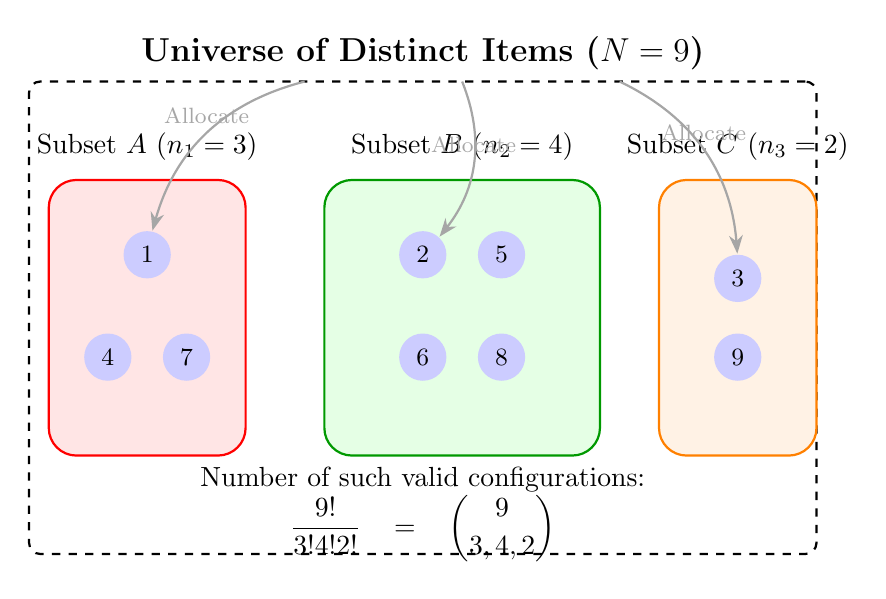
\begin{tikzpicture}[
    >=Stealth,
    node distance=2.5cm,
    thick,
    element/.style={circle, fill=blue!20, minimum size=6mm, inner sep=0pt, font=\small},
    subset/.style={rounded corners=10pt, draw, fill=gray!5, inner sep=10pt}
]

    % Universal Set Bounds
    \node[draw, dashed, rounded corners, minimum width=10cm, minimum height=6cm, label={[font=\large\bfseries]90:Universe of Distinct Items ($N=9$)}] (universe) at (2,0) {};

    % Subsets
    \node[subset, fill=red!10, draw=red, minimum width=2.5cm, minimum height=3.5cm] (A) at (-1.5, 0) {};
    \node[above=0.1cm of A] {Subset $A$ ($n_1=3$)};

    \node[subset, fill=green!10, draw=green!60!black, minimum width=3.5cm, minimum height=3.5cm] (B) at (2.5, 0) {};
    \node[above=0.1cm of B] {Subset $B$ ($n_2=4$)};

    \node[subset, fill=orange!10, draw=orange, minimum width=2cm, minimum height=3.5cm] (C) at (6, 0) {};
    \node[above=0.1cm of C] {Subset $C$ ($n_3=2$)};

    % Elements in A
    \node[element] (a1) at (-1.5, 0.8) {1};
    \node[element] (a2) at (-2, -0.5) {4};
    \node[element] (a3) at (-1, -0.5) {7};

    % Elements in B
    \node[element] (b1) at (2, 0.8) {2};
    \node[element] (b2) at (3, 0.8) {5};
    \node[element] (b3) at (2, -0.5) {6};
    \node[element] (b4) at (3, -0.5) {8};

    % Elements in C
    \node[element] (c1) at (6, 0.5) {3};
    \node[element] (c2) at (6, -0.5) {9};

    % Mappings/Arrows (abstractly showing distribution)
    \draw[->, gray!70] (0.5, 3) to[bend right] node[above, font=\footnotesize] {Allocate} (a1);
    \draw[->, gray!70] (2.5, 3) to[bend left] node[above, font=\footnotesize] {Allocate} (b1);
    \draw[->, gray!70] (4.5, 3) to[bend left] node[above, font=\footnotesize] {Allocate} (c1);

    \node[text width=8cm, align=center] at (2, -2.5) {Number of such valid configurations: \\ $ \displaystyle \frac{9!}{3! 4! 2!} = \binom{9}{3, 4, 2} $};

\end{tikzpicture}
\end{center}

\subsection{Heuristics \& "Cheats"}
\begin{itemize}
    \item \textbf{The "Does Order Matter" Matrix:} 
    \begin{itemize}
        \item Distinct objects, Order matters $\implies$ Permutations ($P^n_r$).
        \item Distinct objects, Order irrelevant $\implies$ Combinations ($C^n_r$).
        \item Indistinguishable objects, distinguishable bins $\implies$ Stars and Bars (see Part 7).
    \end{itemize}
    \item \textbf{Word Translation Cheat:} "AND" translates to multiplication ($\times$) of combinations. "OR" translates to addition ($+$) of combinations.
\end{itemize}

\subsection{Pitfalls \& Fallacies}
\begin{itemize}
    \item \textbf{Overcounting in Combinations:} A fatal mistake is arbitrarily ordering sets that do not have order. For example, if asked to draw two pairs in poker, calculating $\binom{13}{1}\binom{4}{2} \times \binom{12}{1}\binom{4}{2}$ counts "Pair of Aces, Pair of Kings" as distinct from "Pair of Kings, Pair of Aces". The correct approach forces a subset selection of the ranks concurrently: $\binom{13}{2} \binom{4}{2}^2$.
    \item \textbf{Assuming Equiprobability in Heterogeneous Sets:} Assuming $\Prob(\text{win}) = 1/2$ because there are two outcomes ("win" and "lose") without rigorously checking the underlying event cardinalities.
\end{itemize}

\newpage
% ==============================================================================
% PART 5: Conceptual Synthesis and The "Big Picture"
% ==============================================================================
\section{Part 5: Conceptual Synthesis and The "Big Picture"}

\subsection{A) Thematic Connections}
The ultimate theme of this chapter is \textbf{Finite Measure Evaluation via Bijections}. We are establishing isomorphisms between complex compound events (like drawing specific poker hands or distributing heterogeneous laborers) and algebraically simple domains (integer counting problems). By reducing arbitrary probability questions into subset size logic ($\sigma$-algebra cardinality), we unify discrete mathematics with probability theory.

\subsection{B) Forward and Backward Links}
\textbf{Backward Link:} This chapter relies heavily on naive set theory limits (unions, intersections, De Morgan's laws). 
\textbf{Forward Link:} Understanding combinatorial sample spaces is the indispensable bedrock for evaluating discrete \textbf{Random Variables} (Chapter 3), particularly the Binomial, Hypergeometric, and Poisson distributions. Later, as $N \to \infty$, these finite combinatorial fractions morph via Stirling's Approximation into the continuous Gaussian integrals of \textbf{Brownian Motion} and measure-theoretic stochastic calculus. 

% ==============================================================================
% PART 6: Abstract Real-World Modeling (AI, ML, & Quant Finance)
% ==============================================================================
\section{Part 6: Abstract Real-World Modeling}

\subsection{A) Concrete Scenarios}
\begin{enumerate}
    \item \textbf{Generative AI / NLP (Bag of Words \& Multinomial Naive Bayes):} When classifying text sentiments or spam, documents are treated as multi-sets of words. Evaluating the probability of a document given a language model strictly utilizes multinomial combinatorial logic, counting the ways an $N$-length document can be arranged given vocabulary counts.
    \item \textbf{Quantitative Finance (Limit Order Book State Entropy):} In high-frequency algorithmic trading, the limit order book consists of queues of discrete orders at different price levels. Modeling the transition probability of the book's state involves partitioning identical market orders into price bins, essentially modeling entropy using combinatorial partitioning.
\end{enumerate}

\subsection{B) Model Problem Setup: Multinomial Naive Bayes in AI}
We construct a rigorous mathematical model for classifying a document $D$ into a predefined class $C \in \{c_1, c_2, \dots, c_K\}$ (e.g., Spam vs Not Spam).
\begin{itemize}
    \item \textbf{State Space Definition:} Let $\mathcal{V}$ be a finite vocabulary set of size $V$. A document $D$ of fixed length $N$ is modeled as a sequence of discrete random variables $W_1, W_2, \dots, W_N$, where $W_j \in \mathcal{V}$.
    \item \textbf{Order Indistinguishability (Bag of Words):} We assume exchangeability of words. Thus, we map the ordered sequence to a vector of term counts $X = \langle x_1, x_2, \dots, x_V \rangle$, representing the number of times word $v_i$ appears. The deterministic constraint is $\sum_{i=1}^V x_i = N$.
    \item \textbf{Combinatorial Measure:} The number of distinct ordered documents that map to a single count vector $X$ is exactly the multinomial coefficient $\binom{N}{x_1, x_2, \dots, x_V}$.
    \item \textbf{Probability Distribution Setup:} Given a class $C = c_k$, let the generative probability of observing word $v_i$ be $\theta_{ki}$, where $\sum_{i} \theta_{ki} = 1$. Assuming conditional independence of word generation, the probability of observing the specific count vector $X$ given $C=c_k$ is governed by the Multinomial probability mass function:
    \[
    \Prob(X \mid C=c_k) = \frac{N!}{x_1! x_2! \dots x_V!} \prod_{i=1}^V (\theta_{ki})^{x_i}
    \]
    \item \textbf{Optimization (Loss Function):} To train this model, we seek parameters $\Theta$ that maximize the log-likelihood of our training corpus. The negative log-likelihood (Cross-Entropy loss) to minimize is:
    \[
    \mathcal{L}(\Theta) = - \sum_{j=1}^M \left[ \log \left( \frac{N^{(j)}!}{\prod x_i^{(j)}!} \right) + \sum_{i=1}^V x_i^{(j)} \log(\theta_{ki}) \right]
    \]
    The factorial combinatorial term $\log(N!/\prod x_i!)$ acts as a massive normalizing constant that can be ignored during the gradient descent optimization of $\theta_{ki}$, proving how fundamental counting factors isolate strictly from probability continuous parameters in ML models.
\end{itemize}

\newpage
% ==============================================================================
% PART 7: Common Variations and Untested Concepts
% ==============================================================================
\section{Part 7: Common Variations and Untested Concepts}
\subsection{The "Missing" Concept: Indistinguishable Objects in Distinguishable Bins (Stars and Bars)}
The textbook's theorem boxes focus entirely on \textit{distinguishable} objects being partitioned. A major gap in standard probability courses is allocating \textit{indistinguishable} objects into distinguishable bins (equivalent to Bose-Einstein statistics in quantum mechanics).

\begin{theorem}[Stars and Bars / Combinations with Repetition]
The number of distinct ways to distribute $n$ identical, indistinguishable objects into $k$ distinct, distinguishable bins is equivalent to the number of non-negative integer solutions to the equation:
\[
x_1 + x_2 + \dots + x_k = n \quad (x_i \ge 0)
\]
This cardinality is precisely bounded by the binomial coefficient:
\[
\binom{n+k-1}{k-1}
\]
\end{theorem}

\begin{proof}[Rigorous Combinatorial Argument]
Represent the $n$ indistinguishable objects as identical "stars" ($\star$). To divide these stars into $k$ distinguishable bins, we need $k-1$ identical "bars" ($|$) acting as dividers. 
For example, if $n=5$ and $k=3$, the sequence $\star \star | \star | \star \star$ denotes $x_1=2, x_2=1, x_3=2$. 
The mathematical object we are constructing is an ordered sequence of length $N = n + (k-1)$, composed strictly of two distinct equivalence classes of symbols: $n$ stars and $k-1$ bars. 
The number of unique configurations is the number of ways to choose the $(k-1)$ positions for the bars out of the total $n+k-1$ available positions. This is exactly the combination definition:
\[
\binom{n+k-1}{k-1}
\]
The mapping is isomorphic, and the proof holds. $\blacksquare$
\end{proof}

% ==============================================================================
% PART 8: Advanced Diagnostic Testing: "Find the Flaw"
% ==============================================================================
\section{Part 8: Advanced Diagnostic Testing: "Find the Flaw"}
Below are 5 "proofs" or solutions that appear mathematically rigorous but contain a fatal logical, combinatorial, or measure-theoretic flaw. Act as the grader, diagnose the error, and reference the underlying axiom violated.

\subsection{The Flawed Problems}
\textbf{Problem 1 (Algebraic Combinatorics):} "Prove" that $\binom{n}{k} = \binom{n-1}{k} + \binom{n-1}{k+1}$.
\begin{proof}[Flawed Proof]
By Pascal's Identity, we know that to form a committee of size $k$ from $n$ people, we can look at a specific person, Bob. Either Bob is not on the committee, in which case we must select all $k$ members from the remaining $n-1$ people, which is $\binom{n-1}{k}$. Or, Bob is on the committee, meaning we need to select $k+1$ members from the remaining $n-1$ people to ensure Bob isn't lonely, giving $\binom{n-1}{k+1}$. Adding the disjoint cases yields the result. $\blacksquare$
\end{proof}

\textbf{Problem 2 (Probability Space Setup):} An urn contains 3 Red balls and 2 Blue balls. What is the probability of drawing 2 Red balls (without replacement)?
\begin{proof}[Flawed Solution]
Let the sample space of possible outcomes regarding colors be $\sample = \{\text{Red-Red, Red-Blue, Blue-Red, Blue-Blue}\}$. There are 4 possible color combinations. The event $A$ is drawing 2 Red balls. There is exactly 1 way this occurs: "Red-Red". Thus, $\Prob(A) = \frac{|A|}{|\sample|} = \frac{1}{4}$. $\blacksquare$
\end{proof}

\textbf{Problem 3 (Overcounting in Partitions):} A standard 52-card deck is dealt into a 5-card poker hand. What is the total number of distinct hands that contain "Two Pair" (e.g., Two 8s, Two Kings, and one other card)?
\begin{proof}[Flawed Solution]
There are 13 possible card ranks. We choose the first pair's rank in $\binom{13}{1}$ ways. From the 4 suits, we choose 2 suits in $\binom{4}{2}$ ways. We choose the second pair's rank from the remaining 12 in $\binom{12}{1}$ ways, and its suits in $\binom{4}{2}$ ways. Finally, we choose the 5th card from the remaining 44 cards in $\binom{44}{1}$ ways. 
Total configurations = $\binom{13}{1} \binom{4}{2} \binom{12}{1} \binom{4}{2} \binom{44}{1} = 247,104$. $\blacksquare$
\end{proof}

\textbf{Problem 4 (Measure Sub-Additivity Violation):} Two dice are rolled. Event $A$ is "rolling at least one 6". Event $B$ is "the sum is 7". What is the probability of $A \cup B$?
\begin{proof}[Flawed Solution]
For $A$: the probability of a 6 on die 1 is $1/6$, and on die 2 is $1/6$. Thus $\Prob(A) = 1/6 + 1/6 = 2/6$. 
For $B$: The sum of 7 has combinations (1,6), (2,5), (3,4), (4,3), (5,2), (6,1). Thus $\Prob(B) = 6/36 = 1/6$.
By Kolmogorov's Additivity axiom, $\Prob(A \cup B) = \Prob(A) + \Prob(B) = \frac{2}{6} + \frac{1}{6} = \frac{1}{2}$. $\blacksquare$
\end{proof}

\textbf{Problem 5 (Stars and Bars Misapplication):} Find the number of strictly positive integer solutions ($x_i \ge 1$) to the equation $x_1 + x_2 + x_3 = 10$. 
\begin{proof}[Flawed Solution]
This is exactly the formulation for distributing indistinguishable objects into distinguishable bins. We have $n=10$ "stars" and $k=3$ "bins", requiring $k-1 = 2$ "bars". According to the Stars and Bars theorem, the total number of configurations is given by $\binom{n+k-1}{k-1} = \binom{10+3-1}{3-1} = \binom{12}{2} = 66$. $\blacksquare$
\end{proof}

\vspace{1cm}
\subsection{Solution Key (Diagnostic Resolutions)}

\textbf{Resolution 1:} 
\textit{Flaw:} The semantic reasoning contradicts the constraints. If Bob is on the committee of size $k$, he already occupies $1$ spot. The remaining spots to fill are $k-1$, not $k+1$. 
\textit{Correction:} The true identity is Pascal's rule: $\binom{n}{k} = \binom{n-1}{k} + \binom{n-1}{k-1}$. The algebraic addition in the flawed proof will result in an invalid unequal equation.

\textbf{Resolution 2:}
\textit{Flaw:} The sample space $\sample$ proposed does not possess the property of equiprobability, making the formula $\Prob(A) = |A|/|\sample|$ a catastrophic measure-theoretic violation. "Red-Red" is vastly more probable than "Blue-Blue" due to the asymmetric initial constraints.
\textit{Correction:} The true sample space involves combinations of individual distinct balls. $|\sample| = \binom{5}{2} = 10$. The event $A$ is drawing 2 from the 3 Red balls, $|A| = \binom{3}{2} = 3$. The true probability is $\frac{3}{10}$.

\textbf{Resolution 3:}
\textit{Flaw:} Massive overcounting due to symmetric ranking. By using $\binom{13}{1} \times \binom{12}{1}$, the "first" pair and "second" pair are falsely treated as distinguishable subsets. A hand of (8, 8, K, K, 2) is counted once when 8 is selected first, and a second time when K is selected first.
\textit{Correction:} Choose both ranks simultaneously as a subset of 2 out of 13: $\binom{13}{2} \binom{4}{2} \binom{4}{2} \binom{44}{1} = 123,552$.

\textbf{Resolution 4:}
\textit{Flaw:} Multiple Axiom Violations. First, $\Prob(A) \ne 1/6 + 1/6$. Rolling a 6 on die 1 and die 2 are not mutually exclusive events; their intersection $(6,6)$ is double-counted. Second, $A$ and $B$ are not mutually exclusive (e.g., (1,6) and (6,1) exist in both). You cannot use the basic additivity axiom without subtracting the intersections.
\textit{Correction:} Use the inclusion-exclusion principle rigorously. $\Prob(A \cup B) = \Prob(A) + \Prob(B) - \Prob(A \cap B)$.

\textbf{Resolution 5:}
\textit{Flaw:} The theorem $\binom{n+k-1}{k-1}$ explicitly applies strictly to \textbf{non-negative} solutions ($x_i \ge 0$). The problem asks for \textbf{strictly positive} solutions ($x_i \ge 1$). 
\textit{Correction:} Pre-allocate 1 unit to each of the 3 bins to satisfy the strict positivity requirement. This leaves $n' = 10 - 3 = 7$ units to distribute freely (now allowing zero). Applying the theorem on the new $n'$ yields $\binom{7+3-1}{3-1} = \binom{9}{2} = 36$.

\end{document}